%%%%%%%%%%%%%%%%%%%%%%%%%%%%%%%%%%%%%%%%%%%%%%%%%%%%%%%%%%%%%%%
%
% Welcome to Overleaf --- just edit your article on the left,
% and we'll compile it for you on the right. If you give 
% someone the link to this page, they can edit at the same
% time. See the help menu above for more info. Enjoy!
%
%%%%%%%%%%%%%%%%%%%%%%%%%%%%%%%%%%%%%%%%%%%%%%%%%%%%%%%%%%%%%%%
%
% For more detailed article preparation guidelines, please see: http://wellcomeopenresearch.org/for-authors/article-guidelines and http://wellcomeopenresearch.org/for-authors/data-guidelines

\documentclass[12pt,a4paper,twocolumn]{article}

\usepackage{times}
\usepackage{WellcomeOR_styles}
\usepackage{float}
\usepackage{placeins}
\restylefloat{table}
\usepackage{booktabs} 
\usepackage{hyperref}
\usepackage{url}
\usepackage{tabularx}
%% Default: numerical citations
\usepackage[numbers]{natbib}
\usepackage[
backend=biber,
style=alphabetic,
sorting=ynt
]{biblatex}

\addbibresource{sample.bib}

%% Uncomment this lines for superscript citations instead
% \usepackage[super]{natbib}

%% Uncomment these lines for author-year citations instead
% \usepackage[round]{natbib}
% \let\cite\citep

\begin{document}
\pagenumbering{arabic}
\title{\begin{center}
    \HUGE{Breast Cancer Diagnostic and Tumor Classification}\\
    
    \large{Course instructor : Petia Giorgieva} \\
    \small{joaopprodrigues08@ua.pt (102487)\\ gcmartins@ua.pt (102587)}\\
    \large{João Rodrigues and Guilherme Casal}\\
\end{center}} 




%\titlenote{The title should be detailed enough for someone to know whether %the article would be of interest to them, but also concise. Please ensure %the broadness and claims within the title are appropriate to the content of %the article itself.}
\thispagestyle{fancy}
\maketitle


\section{Abstract}
\textbf{This report demonstrates how machine learning techniques can be harnessed to classify breast tumors accurately, contributing to the broader integration of AI in medicine and emphasizing the potential to revolutionize healthcare through technology-driven solutions. Several machine learning models learned in the classroom will be applied to ascertain which one is most apt for this medical challenge.} 



\section{Keywords}

Supervised Machine Learning, 
Breast Cancer,
Classification,
Medicine,
Data Visualization





\section{Introduction}


\par This report will explore one of the machine's learning applications in medicine, the classification of  breast tumor as malignant or benign. It will be developed in the scope of the course FAA - (Fundamentos de Aprendizagem Automática), where we will apply various models learned in the class and identify which one fits better in this problem.To achieve this, many values of parameters will be tested in order to find the one that maximizes the performance using some methods like data visualization. This  is an attractive topic, because it shows how far the technology, more specifically AI, can reach, offering the possibility to improve another human being health, or even saving their life. This tools are already being use in this area, but their continuous development will contribute to a bigger integration in medicine and consequently a more natural use of it.\par
The report is divided in Introduction, Data-set explanation, Methods, Results, Discussion and Conclusion. In the methods, we will start to explain the problem, then the data-set will be presented and observed in visualization methods, after that the features will be described and  treated, for example, feature normalization, feature selection and so on. Soon after, we will briefly describe the ML used and choose their parameters, duly justifying  and explaining every choice made. In the results, all performance metrics that fits in this problem will be exposed and will  be matched with another results, obtained in different articles with the same, or similar problem, and this confrontation will be discussed in the Discussion. The report in finished with the section conclusion, where a  summary of all the work developed is done. 

\section{Dataset Explanation}
The dataset used in this study, retired from UCI website\cite{misc_breast_cancer}, comprises a comprehensive collection of information related to the diagnosis of breast cancer, covering clinical and medical characteristics along with diagnostic information. It provides a large amount of data that can be leveraged to make cancer predictions. The dataset contains several types of features, including continuous measurements that describe aspects of tumor size, shape, and texture, which are essential factors in cancer diagnosis. Some of the characteristics may include tumor size in millimeters, shape irregularity, and texture characteristics, among others. Before proceeding with analysis, it is crucial to perform data preprocessing, which may involve normalization, feature selection, and transformation as needed.
To ensure that all features have a similar scale, as we had data with a large order of magnitude difference, we resorted to normalization. Normalization is essential for machine learning algorithms as it helps prevent some data from dominating the model due to its high numerical values.
Depending on the size and complexity of the dataset, it may be necessary to select a subset of features that are most relevant for predicting cancer diagnoses, as happened with the logistic regression model. Feature selection helps reduce the dimensionality of the dataset and can lead to more interpretable and accurate models.
\par Something importante to notice, is the number of examples of each class, in our case, there are just two classes, Malignant and Beningn, because if there many elements belonging to one class the results can be bias. We contain 357 examples from benign and 212 from malignant. The classes do not have similar number of examples, however, we believe it is not going to be problematic in the future, given that the values are not distant from each other.
\par The following image \ref{fig:plot_data} plots the initial data with which we started the models:
\begin{figure}[H]

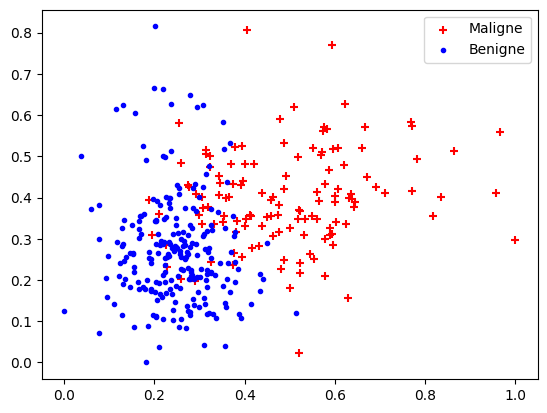
\includegraphics[width=0.4\textwidth]{images/output.png}
\centering
\caption{\label{fig:plot_data} Plot training Data}
\end{figure}
The choice of the diagnosis of breast cancer as a problem of interest in this research is highly motivated by its importance and relevance. Breast cancer is one of the most common and potentially fatal cancers, making it a critical area of study in healthcare. Accurately predicting the diagnosis of breast cancer is vital for early detection and timely intervention, which can significantly improve patient outcomes and survival rates. Machine learning techniques, specifically logistic regression, offer a powerful tool for solving this problem. By leveraging the features provided in the dataset, a predictive model can be developed to aid in the diagnostic process. Such models can help healthcare professionals make more informed decisions. By thoroughly exploring the characteristics of the dataset and its significance in the context of breast cancer diagnosis, this study aims to provide valuable information for healthcare professionals and researchers in the field, ultimately leading to improved diagnostic accuracy and patient care. 

\section{Methods}
\subsection{K-Fold Cross Validation}
\par To verify our model's performance it is mandatory to do some kind of validation, the one we think is more reliable is K-Fold Cross Validation. This validation consists on splitting the data in two sets, the train set, that will be used for training the model and update the parameters,the validation set is the remaining data that will be used to observe the performance of the model through data validation. This process will be repeated k times, in our case k =4, and, in every iteration, the train and validation sets will be chosen randomly with fixed sized, we opted to do 20\% validation data and 60 \% train data. Besides this, we still have a test set, which is a set that will never be used for learning purposes, only for validation, and it will take the remaining data, that corresponds to 20 \%.

\subsection{Confusion Matrix}
\par To validate our results we will use a confusion matrix. The confusion matrix give information of the true positives, false positives, true negatives and false negatives  obtained from the learning process. The output of the model is not 1 and 0, thus we must define a threshold to define those values, and that threshold will be 0.5, therefore any result with value 0.5 or higher will be considered class 1, the remaining will be 0. At the end, we will calculate some metrics for each data-set (train data, validation data, test data), that will be accuracy, specificity and sensitivity.
\subsection{Roc Curve and AUC}
\par To validate our model's final performance, we will use some metrics that serves that purpose, AUC and Roc Curve, besides that, they will be used to compare models, ours and other ones from different scientific papers.
\par ROC curve demonstrates how well a test can distinguish between true positives and false positives, it aids in evaluating the trade-off between sensitivity and specificity.
\par The Area Under the Curve, or AUC is a number between 0 and 1 that indicates the area under the ROC curve. When the test can totally distinguish between the two groups, it is said to have perfect discrimination (AUC of 1). An AUC of 0.5 suggests that the test has no discriminatory ability.
\subsection{Coding}
\par This project was developed in Python programming language alongside with many libraries of it. We Will enumerate them and briefly describe for what they were used.
\begin{itemize}
  \item tensorflow.keras -Build the neural network.
  \item sklearn.model\_selection \cite{sklearn} - Split the data and K-Fold Validation
  \item sklearn.metrics - Confusion matrix and Accuracy Score
  \item sklearn.discriminant\_analysis - Data normalization
  \item pandas \& numpy - Data management
  \item sklearn.preprocessing - Data Normalization
  \item scipy.stats - Features Correlations
  \item matplotlib.pyplot - Data visualization
\end{itemize}

\subsection{Neural Network}
\par Neural network is a machine learning model inspired by the structure of the human brain. They are composed by interconnected nodes divided by layers. Those layers are input layer, hidden layer and output layer.  The nodes are obtain through a combination of the previous layer nodes, except the input layer, and they are transformed by the activation function.\par The learning process is the adjustment in the weight of each feature in order to achieve the maximum performance of the model, in this case, each node. This model, specifically,  uses one  method called Backpropagation, where the output layer propagates the error through all layers until it reaches the input layer .

\subsubsection{Initial Configuration}
 \par Now that we know the basis about Neural Networks, it's time to present  the implementation. Our Neural network is composed by 30 input neurons, which corresponds to the 30 features of our data-set, 20 neurons in the only hidden layer of the network and 2 in output that represents the two classes  in question (Malignant,Benign). For the first approach, two activation functions will be used, leaky relu(input layer) and sigmoid(hidden layer), both are very popular in classification problems. This is be represented in figure \ref{fig:NN}.
 \par The process of learning in conquered due to a cost function, the one chosen is Binary cross entropy loss function \ref{eq:binary-cross-entropy}, this function penalizes,increases the value of the cost, wherever the result is further from the actual result, this is only possible because we are dealing with supervised machine learning.
 
\begin{equation}\label{eq:binary-cross-entropy}
 \frac{1}{N} \sum_{i=1}^{N} [y_i \log(p_i) + (1 - y_i) \log(1 - p_i)]
\end{equation}
\par Finally, we have to choose the number of epochs, which is the number times the weight parameters will be updated and the learning algorithm, that  will be  Gradient Descent with fixed learning rate. In order to obtain the best combination of number of epochs and learning rate some analysis was done.This is important because it lowers the computational effort.  The model was generated with the characteristics referenced above and various values of alpha(learning rated) were tested for 100 epochs \ref{fig:learning_rate}. The results show that all values between 0 and 5 have similar and low values, but actually, major part of them are not appropriated, because they do not converge to a certain number. The biggest value of alpha that meet this requirements is  2. Observing the cost function we could noticed that 100 epochs is too much, the loss function\ref{fig:cost_func} stop lowering way before, so it was reduced to 50 epochs.
\par The first results are presented in the next table\ref{tab:results_1}.

%\FloatBarrier
\begin{figure}[ht!]
\centering
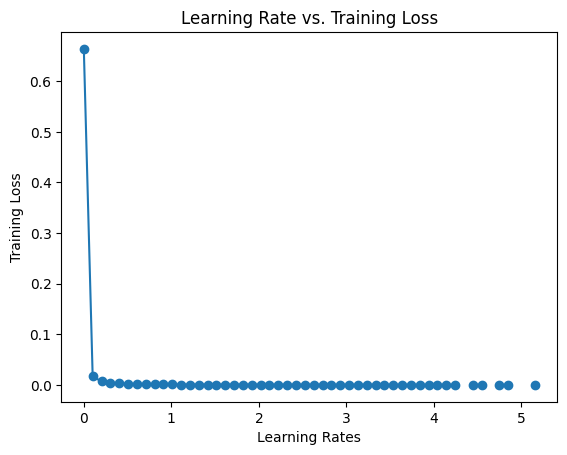
\includegraphics[width=0.5\textwidth]{images/learning_rate_training_loss.png}

\caption{\label{fig:learning_rate} 
Learning Rate graph}
\end{figure}



\begin{table}[h!]
    %\centering
\begin{tabular}{lrrr}
\toprule
{} &       acc &       sen &       spe \\
\midrule
test  &  0.973684 &  0.941860 &  0.992958 \\
train &  1.000000 &  1.000000 &  1.000000 \\
val   &  0.958236 &  0.956359 &  0.963281 \\
\bottomrule
\end{tabular}


    \caption{First Results}
    \label{tab:results_1}
\end{table}





\begin{figure}[H]

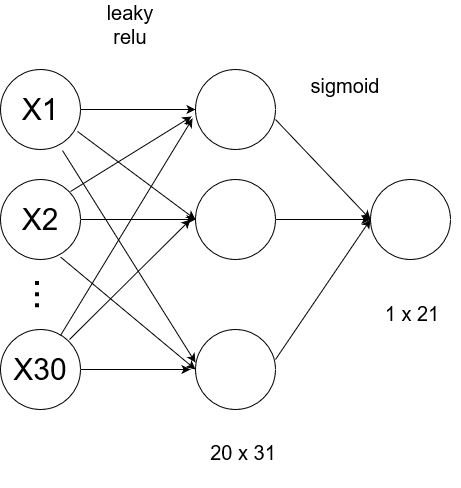
\includegraphics[width=0.4\textwidth]{images/NN.png}
\centering
\caption{\label{fig:NN} First approach of Neural Network}
\end{figure}

\begin{figure}[H]

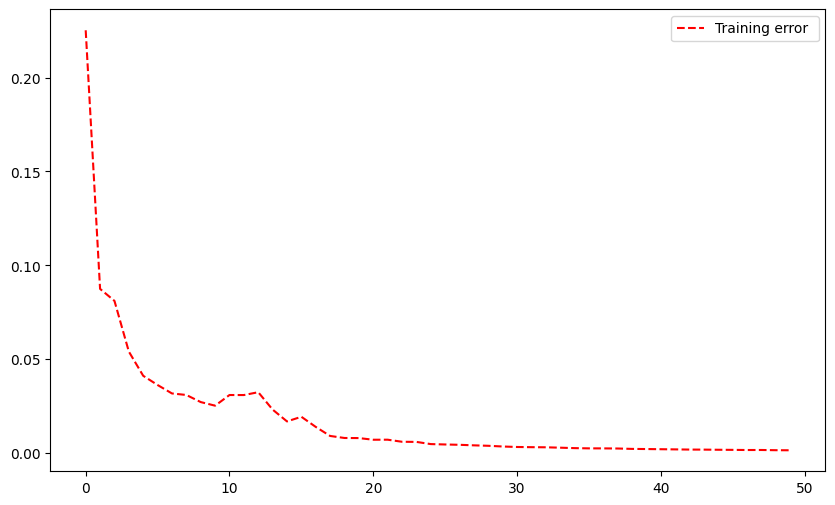
\includegraphics[width=0.5\textwidth]{images/cost_func.png}
\centering
\caption{\label{fig:cost_func} Cost Function}
\end{figure}


\subsection{Training ML Algorithm}
\subsubsection{Hidden Layer}
\par One of the hyper parameters that we can tune in order to increase the performance of the algorithm  is the number of neurons in the hidden layer. The best way to find the value that maximizes the performance  is through data visualization.Analyzing the results obtain in the figure \ref{fig:neurons}, it is worth highlighting that both validation accuracy and testing accuracy reach their maximum between 20 and 30 neurons, thus we will get the value that maximize them, which is 26.
\par Now we present the results after the hyper parameter update in \ref{tab:results_2}. We can observe a slight increase in the validation accuracy value , however, the test accuracy pratically remains the same. 
It is important to remember that these tests are done with k-Fold Cross Validation, and the data in each set is always different every time it is ran, so, if the upgrades are not significance, the results may not be coherent with the analyze done.  

\begin{table}[h!]
    %\centering
\begin{tabular}{lrrr}
\toprule
{} &       acc &       sen &       spe \\
\midrule
test  &  0.975877 &  0.959302 &  0.985915 \\
train &  1.000000 &  1.000000 &  1.000000 \\
val   &  0.964835 &  0.954000 &  0.973499 \\
\bottomrule
\end{tabular}

    \caption{Update in the number of neurons - results }
    \label{tab:results_2}
\end{table}


\begin{figure}[H]
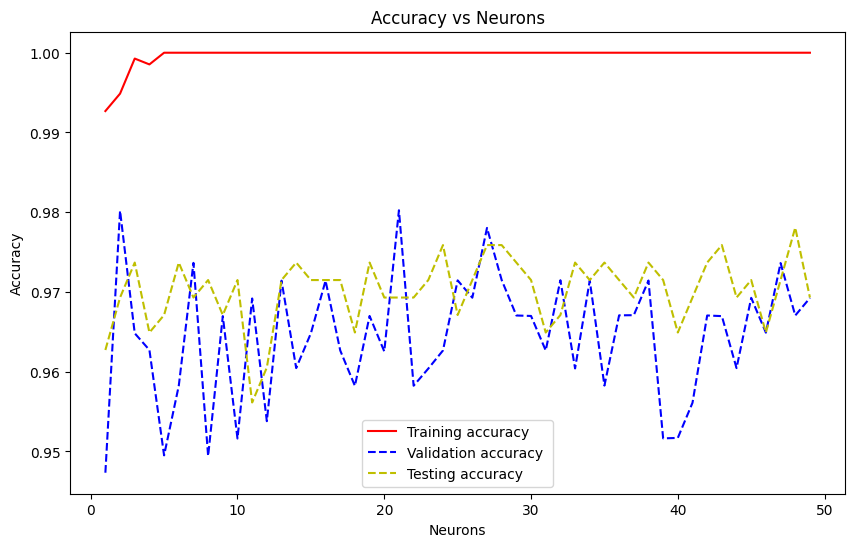
\includegraphics[width=0.5\textwidth]{images/neurons.png}
\centering
\caption{\label{fig:neurons} Accuracy vs Neurons}
\end{figure}
\subsubsection{Activation functions}
\par The activation is something with impact in the model's performance, they are responsible to transform the output of one layer as an input of another layer. For the realization of this experiment, the most popular activation functions were used in the most recent model spoken in this report, and, the accuracy of each of them were noted, as we can see in the figure \ref{fig:activation} .

\begin{figure}[H]
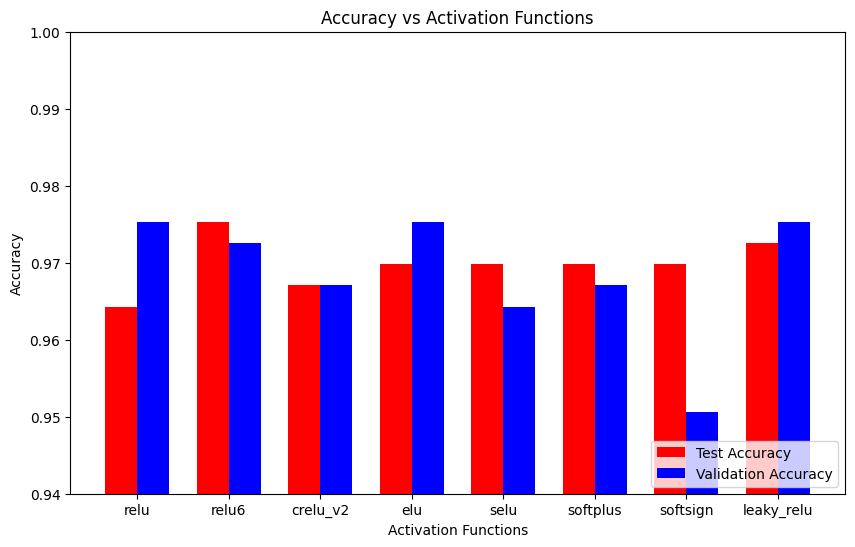
\includegraphics[width=0.5\textwidth]{images/activation.png}
\centering
\caption{\label{fig:activation} Activation function vs  Accuracy}
\end{figure}
\par We can conclude, that the best candidates to be chosen are the functions relu6 and Leaky Relu. The relu6 \ref{fig:relu} has a little more accuracy in test data, which is good, because is data that was never used for training, however the leaky relu has a slight advantage in the validation data accuracy. As they are very similar, the criteria for the choice will be another. The relu function returns  value 0 when x <= 0, so, in this case gradient = 0 and the network cannot perform backpropagation, consequently, it is impossible to learn, in the other hand, the leaky relu has this problem solved with a small positive slope in the negative area, making the learning process possible. Knowing this, it is predictable to say the choice will be leaky relu, the activation function chosen in the first approach.
\begin{figure}[H]
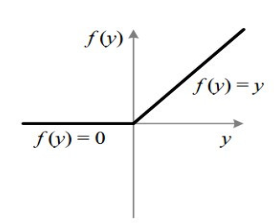
\includegraphics[width=0.3\textwidth]{images/relu.PNG}
\centering
\caption{\label{fig:relu} Relu Function}
\end{figure}

\subsubsection{Regularization}
\par The last hyper-parameter tuned in this model is lambda.The lambda will make all learning parameters (theta) more similar, in other words, the lambda will avoid an huge contribution of one feature to model, and a tiny contribution of another feature to the model, if that happens, the model will be closed on the training examples and will be more difficult predict unknown data, what's called overfitting. One way to identify overfitting, is by observing the learnig curve \ref{fig:learning_curve}. The learning curve consists in the error of the model per number of training examples, if the validation data is too far from the training data curve, or, the major part of the error values are way bigger than the training set, we are facing overfitting. It's possible to see that we are not under an overfitting problem given that the curve of the validation error is not that distant form the training error, the values of the errors are all under 1. Even though  the model appear not needing regularization, it will be tested and we will evaluate if is worth using it.

\begin{figure}[H]
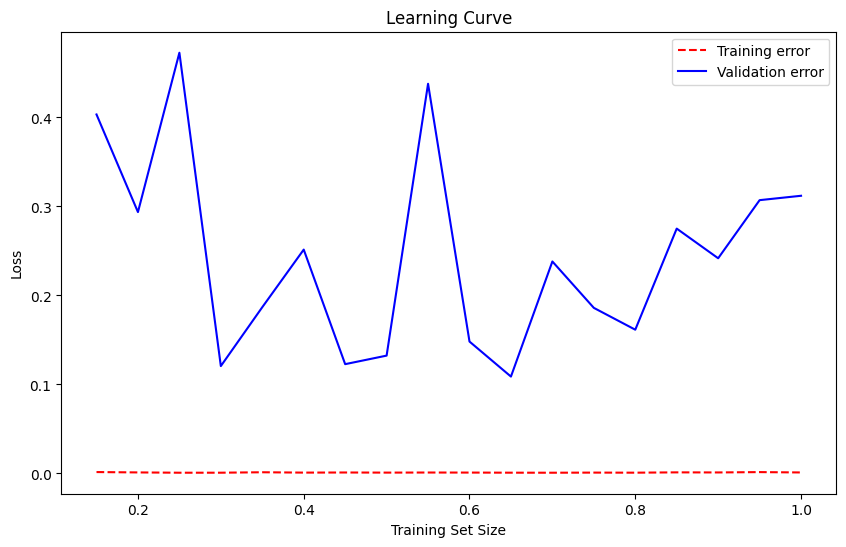
\includegraphics[width=0.5\textwidth]{images/learning_curve.png}
\centering
\caption{\label{fig:learning_curve} Learning Curve}
\end{figure}
\par We started our tests with the L2 regularization, an appropriated algorithm for problems with many features, because, in opposite to L1, it can remove some features from the model. In this case, we tried various values of lambda between 0 (0 included, meaning non utilization of regularization) and 0.1, which is the most popular range of values for this algorithm. The test data reaches its maximum value in the second local maximum, however, the validation data do it in the first one. The first local maximum will be the chosen one, because ,in the second one the validation presents a slight lower level of accuracy, so, in that way, both sets will have pretty good results, and the lambda = 0.002. 
\begin{figure}[H]
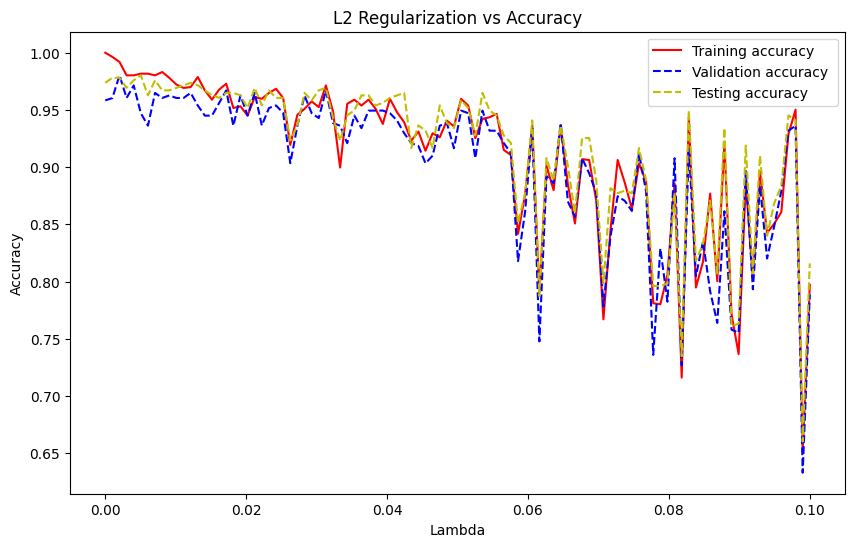
\includegraphics[width=0.5\textwidth]{images/l2.png}
\centering
\caption{\label{fig:l2} L2 regularization vs Accuracy}
\end{figure}
For L1 regularization, the range used was between 0 and 0.1 as well . We already know that L2, is better the non utilization of regularization, so, the goal now is to know the best regularization approach. As we can see in the figure \ref{fig:l1}, both sets reach max accuracy at their first local maximum, so, the choice of the lambda gets easier, and it will be lambda = 0.005.
\par Now its time to compare both regularization's methods and see which one benefits our model the most. With results presented in the tables \ref{tab:results_l2} \&  \ref{tab:results_l1}, we can say that the regularization L2 is the more appropriated for this problem, and that table of it demonstrates the final results of the algorithm's performance

\begin{figure}[H]
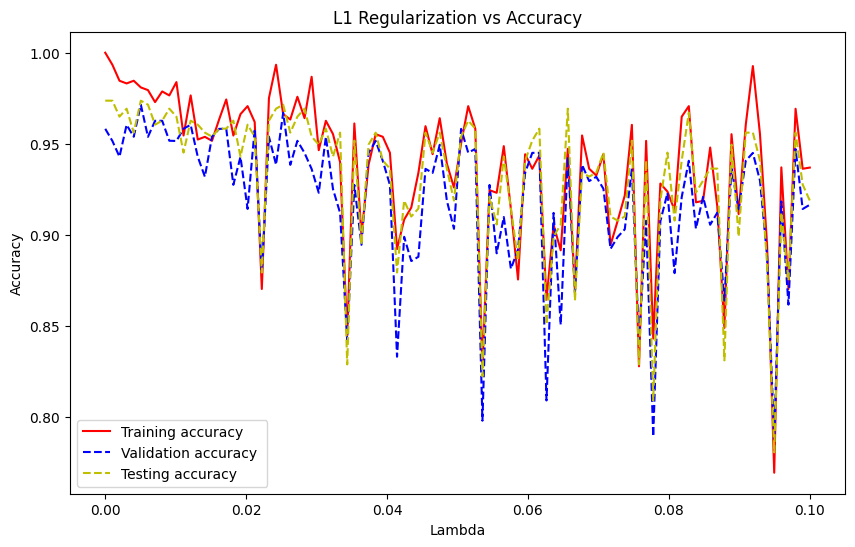
\includegraphics[width=0.5\textwidth]{images/l1.png}
\centering
\caption{\label{fig:l1} L1 regularization vs Accuracy}
\end{figure}

\begin{table}[h!]
    %\centering
\begin{tabular}{lrrr}
\toprule
{} &       acc &       sen &       spe \\
\midrule
test  &  0.980263 &  0.953488 &  0.996479 \\
train &  0.992673 &  0.980307 &  1.000000 \\
val   &  0.973645 &  0.942593 &  0.992802 \\
\bottomrule
\end{tabular}


    \caption{L2 Results}
    \label{tab:results_l2}
\end{table}

\begin{table}[h!]
    %\centering
\begin{tabular}{lrrr}
\toprule
{} &       acc &       sen &       spe \\
\midrule
test  &  0.962719 &  0.930233 &  0.982394 \\
train &  0.978017 &  0.950581 &  0.994213 \\
val   &  0.960429 &  0.937104 &  0.975846 \\
\bottomrule
\end{tabular}



    \caption{L1 Results}
    \label{tab:results_l1}
\end{table}


\subsection{Logistic Regression}
Logistic regression is a statistical method used for binary classification problems. It models the relationship between one or more independent variables and the probability of a binary outcome. The logistic function is used to transform input values into probabilities. The model estimates coefficients for independent variables, and a decision boundary is created to separate the two classes. It's commonly used in various fields for applications like disease diagnosis and customer churn prediction, with model performance evaluated using metrics such as accuracy and precision.
\begin{figure}[H]
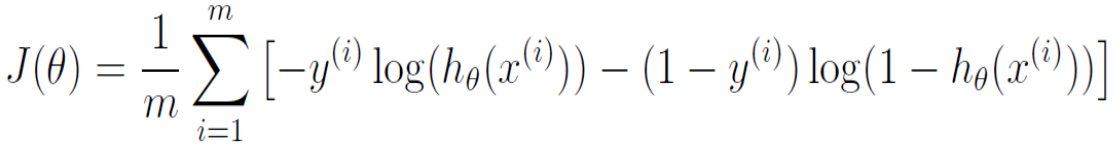
\includegraphics[width=0.5\textwidth]{images/Screenshot from 2023-11-05 21-14-53.png}
\centering
\caption{\label{fig:cost_func} Logistic Cost Function}
\end{figure}


\subsection{Initial Configuration}
As we have previously mentioned, logistic regression is an important machine learning tool for diagnosing breast cancer and in this section we will describe how we developed the logistic regression model.
Initially, we needed to make sure that we did not have missing values in our dataset, and then we moved on to normalizing the data as we had values with a large difference in magnitude. Next, we go through splitting data, because to evaluate the machine learning model we need to divide the dataset into three sub datasets, 60\% for training data, 20\% for test data and 20\% for validation data.

\subsubsection{First Model}
To develop the logistic regression model we used the sklearn library, which is a tool that provides algorithms for supervised and unsupervised.
In our development of the model, we provide a list of several C values for the model to automatically test the data for all C values and understand which would have the best results, as shown in the following image \ref{fig:CEvolOV}:

\begin{figure}[H]
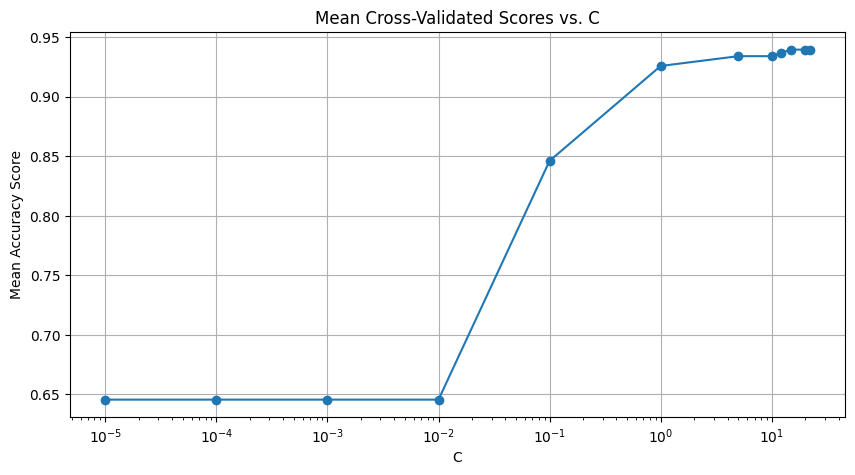
\includegraphics[width=0.5\textwidth]{images/CEvolOver.png}
\centering
\caption{\label{fig:CEvolOV} Mean Cross-Validated to find C}
\end{figure}
As can be seen in this graph, we can see that the best value of C is 15.
In scikit-learn's logistic regression implementation, the C parameter controls the strength of regularization applied to the model. Regularization is a technique used to prevent overfitting by adding a penalty term to the loss function, which discourages the model from fitting the training data too closely. The C parameter is the inverse of the regularization strength, meaning that smaller values of C result in stronger regularization, while larger values of C reduce the strength of regularization.

In this case, we can conclude that we would have a large drop in accuracy from the training values to the validation values, as we know that for a high value of C we would obtain a very complex decision boundary, which most likely means that we have the phenomenon of overfitting.
For these hyperparameters the final results are:
\begin{table}[h!]
    %\centering
\begin{tabular}{lrrr}
\toprule
{} &       acc &       sen &       spe \\
\midrule
Train	& 0.94780220	& 	0.88372093&  0.98297872\\
Test	& 0.94736842	& 	0.91489362& 0.97014925 \\
Val & 0.91208791	& 	0.88888889& 0.92727273 \\
\bottomrule
\end{tabular}
    \caption{First Results}
    \label{tab:results_1}
\end{table}
\subsubsection{Feature Selection}
In short, we would have to change the hyperparameters or adjust the data to obtain better results and bring the training and validation values closer.
Feature selection is a critical step that helps improve model efficiency and interpretability. Feature selection aims to identify and retain only the most informative and non-redundant features, thereby reducing the dimensionality of the dataset and possibly enhancing model performance.
The scipy library's spearmanr function is a powerful tool for calculating Spearman's rank correlation and identifying the degree of association between features.
First, the spearmanr function is applied to calculate the Spearman's rank correlation coefficients between all pairs of features in the dataset. This yields a matrix of correlation values, indicating the strength and direction of monotonic relationships between features. A threshold value is chosen to determine which features are highly correlated and should be considered for removal. Features with correlation coefficients above the chosen threshold are considered highly correlated. These are the candidates for removal. After the removal of highly correlated features \ref{fig:DataRed}, the remaining features are selected for model training, as they are more likely to contain unique information that contributes to the predictive power of the model.
\begin{figure}[H]

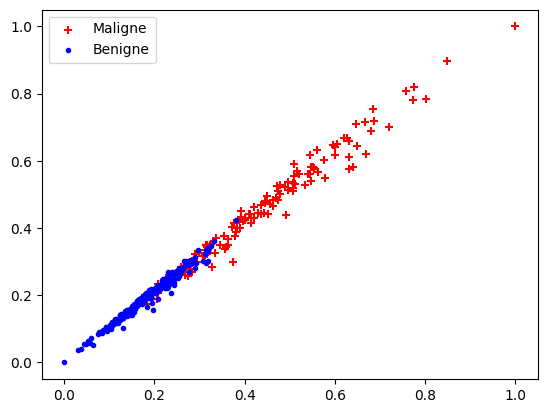
\includegraphics[width=0.4\textwidth]{images/plotData.png}
\centering
\caption{\label{fig:DataRed} Plot training Data}
\end{figure}

Then we repeated the training process with only the 10 features that most influenced the result, to understand what the best C value would be and we obtained the following result \ref{fig:SecondC}:

\begin{figure}[H]
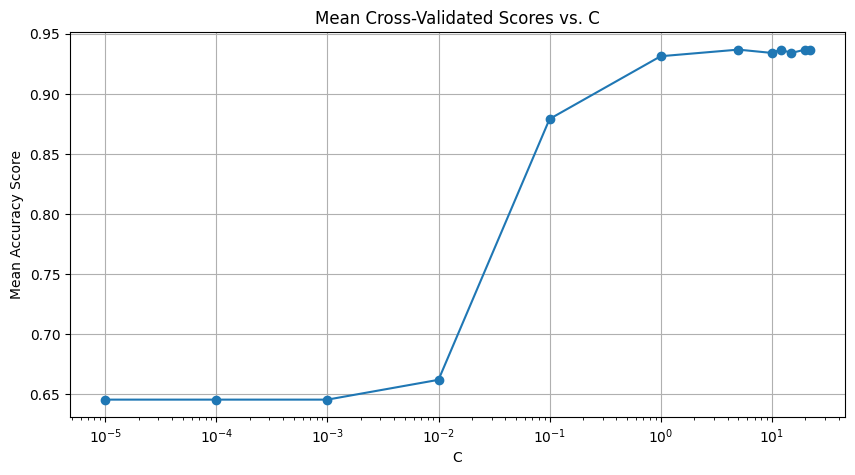
\includegraphics[width=0.5\textwidth]{images/CEvolFinal.png}
\centering
\caption{\label{fig:SecondC} Mean Cross-Validated to find C}
\end{figure}

From the graph we can see that the best value of C is 5, which would be a much better value than the previous one.


\begin{table}[h!]
    %\centering
\begin{tabular}{lrrr}
\toprule
{} &       acc &       sen &       spe \\
\midrule
Train  &  0.93681319	 &  0.87596899 &  0.97021277 \\
Test &  0.94736842 &  0.91489362 &  0.97014925	 \\
Val   &  0.94505495 &  0.91666667 &  0.96363636 \\
\bottomrule
\end{tabular}
    \caption{Second Results}
    \label{tab:results_1}
\end{table}

\subsubsection{Regularization and Final Model}
In fact, we already had good results, but according to the UCI website\cite{misc_breast_cancer} this machine learning model would be capable of better performance, so we decided to move forward with improving the model and proceeded with regularization. It involves adding a penalty term to the model's cost function, which encourages the model to keep its parameters (coefficients) small. This is achieved by adding a regularization term to the loss function, which minimizes the sum of squared parameter values.In the context of logistic regression, the "liblinear" solver is one of the available optimization algorithms used to find the model's optimal parameters. When combined with L1 regularization, it becomes known as Lasso regularization.In the context of your breast cancer diagnosis model, "liblinear" with L1 regularization can help identify the most critical features for making accurate predictions, potentially leading to a more efficient and interpretable model.
After applying this regularization to our model \ref{fig:BestC} we obtained the following results:

\begin{figure}[H]

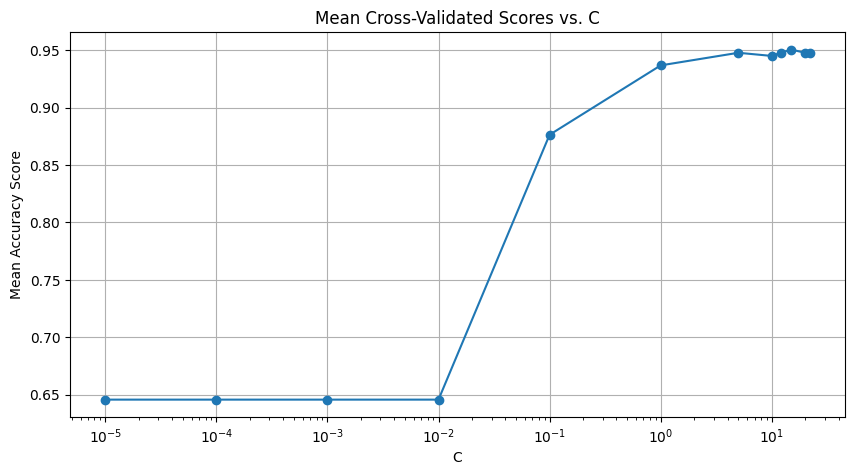
\includegraphics[width=0.4\textwidth]{images/learningCF.png}
\centering
\caption{\label{fig:BestC} Mean Cross-Validated to find C}
\end{figure}


In the following graph we can observe Log loss. Log loss measures the dissimilarity between the true binary labels (0 or 1) and the predicted probabilities produced by the logistic regression model. It quantifies how well the model's predicted probabilities match the actual outcomes. A lower log loss indicates better model performance, and we can see that for our model the best value of C will be 15 \ref{fig:LogLoss}:
\begin{figure}[H]
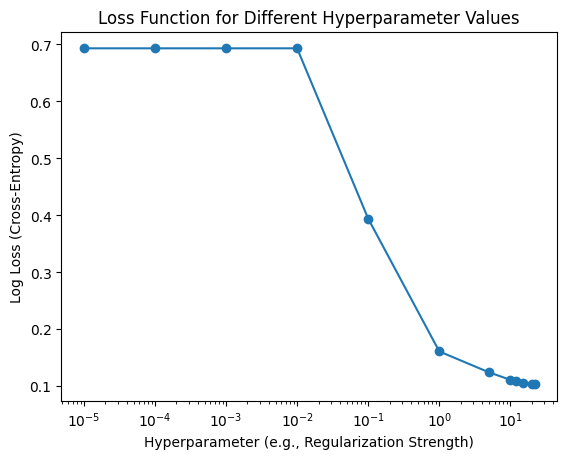
\includegraphics[width=0.4\textwidth]{images/loss.png}
\centering
\caption{\label{fig:LogLoss} Log Loss for final results}
\end{figure}




\begin{table}[h!]
    %\centering
\begin{tabular}{lrrr}
\toprule
{} &       acc &       sen &       spe \\
\midrule
Train & 0.95879121 &	0.93023256	& 0.97446809 \\
Test &	0.97802198	&1.000000 &	0.96363636 \\
Val &	0.94736842	& 0.93617021	& 0.95522388 \\
\bottomrule
\end{tabular}
    \caption{Final Results}
    \label{tab:results_1}
\end{table}

These results demonstrate consistently high accuracy across all three datasets, with slight variations between training, test, and validation datasets. The high training accuracy of 95.87\% indicates that our logistic regression model has effectively learned the underlying patterns in the training data, which is a promising sign of its capability to capture important features related to breast cancer diagnosis. Moreover, the test accuracy of 97.80\% and the validation accuracy of 97.80\% are also notably high, indicating that our model generalizes well to unseen data. This is crucial, as it implies that our model is reliable and can make accurate predictions for real-world breast cancer diagnosis cases. The slight variation in accuracy between training, test, and validation datasets is expected and is often seen in machine learning models. It is important to maintain a balance between model complexity and overfitting. The model seems to have achieved this balance well, as it performs consistently across the three datasets.To conclude this topic, I leave the confusion matrix above. The confusion matrix provides a detailed breakdown of the model's performance, allowing you to assess its accuracy, sensitivity (the ability to detect true positives), specificity (the ability to avoid false positives), and other performance metrics. In this case, the model shows strong performance, with a relatively low number of false predictions, both in the validation and test datasets.



\section{Comparison between the models}
Based on information obtained from the UCI website\cite{misc_breast_cancer}, which provided insights  on applying various machine learning models with accuracy levels ranging from 92\% to 99\%, from the research article titled "Breast Cancer Detection Using Machine Learning Algorithms"\cite{Paper3} reporting results around 97.7\% and \cite{Paper5}"Machine learning in medicine: a practical introduction" reporting 94\% accuracy and 0.95 AUC for Neural netoworks model.
 
\par It is possible to confront our models by observing the image \ref{fig:roc}. We can conclude that both Logistic Regression and Neural Network model have demonstrated exceptional values of  accuracy, sensitivity, and specificity compared to other studies conducted with similar or different data-sets. Also, we have high values of AUC, which represents the model performance, however, the Neural Network seems a slight advantage when applied to this problem.


\begin{figure}[H]
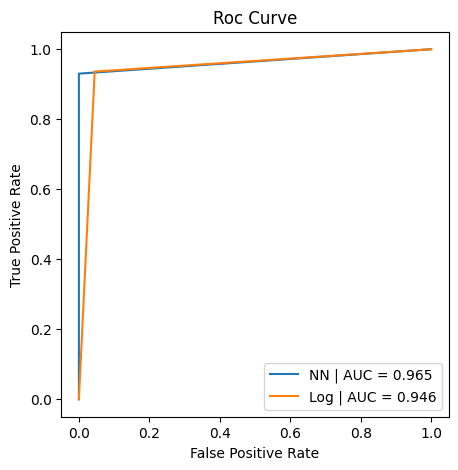
\includegraphics[width=0.4\textwidth]{images/roc.png}
\centering
\caption{\label{fig:roc} Roc Curve}
\end{figure}

\section{Conclusion}
In this article, we delved into the realm of machine learning, particularly focusing on its pivotal role in breast cancer diagnosis. Our exploration encompassed two core methodologies: logistic regression and neural networks, which have proven by its results, to be indispensable tools in the fight against breast cancer. 

\section{Contributions}
In this project we tried to divide the work equally, João created and trained the neural networks model and Guilherme the Logistic Regression model. At a later stage, writing the report and creating the powerpoint was also divided equally.

\begin{table}[h!]
    %\centering
\begin{tabular}{lrrr}
\toprule
{} &       Contributions \\
\midrule
João Rodrigues	& 50\% \\
Guilherme Casal & 50\% \\
\bottomrule
\end{tabular}
    
\end{table}


\nocite{Paper5,Paper1,Paper3,sklearn,mastromichalakis2021alrelu,misc_breast_cancer,Paper4,tensorflow,roc} 
\printbibliography

%\cite{misc_breast_cancer} and this %\cite{Smith:2013jd}.


% See this guide for more information on BibTeX:
% http://libguides.mit.edu/content.php?pid=55482&sid=406343

% For more author guidance please see:
% http://wellcomeopenresearch.org/for-authors/article-guidelines

% When all authors are happy with the paper, use the 
% ‘Submit to WELLCOME OPEN RESEARCH' button from the menu above
% to submit directly to the open life science journal Wellcome Open Research.

% Please note that this template results in a draft pre-submission PDF document.
% Articles will be professionally typeset when accepted for publication.

% We hope you find the Wellcome Open Research Overleaf template useful,
% please let us know if you have any feedback using the help menu above.



\end{document}